\documentclass[journal]{IEEEtran}

\usepackage{amsmath,amsfonts,amssymb}
\usepackage{algorithmic}
\usepackage{algorithm}
\usepackage{array}
\usepackage{textcomp}
\usepackage{stfloats}
\usepackage{url}
\usepackage{verbatim}
\usepackage{graphicx}
\usepackage{cite}
\usepackage{booktabs}
\usepackage{multirow}
\usepackage{tikz}
\usepackage{xcolor}
\usepackage[hidelinks]{hyperref}

% TikZ definition for ORCID badge
\definecolor{lime}{HTML}{A6CE39}
\DeclareRobustCommand{\orcidicon}[1]{%
    \href{https://orcid.org/#1}{%
        
\begin{tikzpicture}[scale=0.18, baseline=-0.3ex]
            \fill[lime] (0,0) circle (1.0);
            \node[white, font=\tiny\sffamily\bfseries] at (0,0) {iD};
        \end{tikzpicture}%
    }%
}

\begin{document}

\title{Decoupled Dual-Stream PatchCL-AE with Parallel Multi-Head Self-Attention Guidance for Unsupervised Medical Image Anomaly Detection}

\author{Cao-Phuc~Ha\,\orcidicon{0009-0004-7024-5166}
        and~Phu-Nguyen~Le$^*$\,\orcidicon{0000-0001-6773-6336},~\IEEEmembership{Member,~IEEE}%
\thanks{This research was supported by the Vietnam Aerospace University during the 2026--2027 academic year.}%
\thanks{Cao-Phuc Ha is with the Department of Artificial Intelligence, FPT University, Ho Chi Minh City 700000, Vietnam (e-mail: caophucai@gmail.com).}%
\thanks{$^*$Phu-Nguyen Le is with the Faculty of Electrical and Electronics Engineering, Vietnam Aerospace University, 104 Nguyen Van Troi Street, Phu Nhuan Ward, Ho Chi Minh City 700000, Vietnam (e-mail: nguyenlp@vaa.edu.vn).}%
\thanks{$^*$Corresponding author: Phu-Nguyen Le.}%
}

% Paper headers
\markboth{IEEE Transactions on Medical Imaging,~Vol.~XX, No.~XX, 2026}%
{Ha and Le: Decoupled Dual-Stream PatchCL-AE for Unsupervised Medical Anomaly Detection}

\maketitle

\begin{abstract}
Patch-wise contrastive learning provides an effective mechanism for unsupervised anomaly detection in medical imaging by enforcing localized spatial correspondence between raw and reconstructed scans. However, contemporary frameworks such as PatchCL-AE exhibit a significant performance limitation when applied to bilaterally symmetric anatomical structures, denoted as the bilateral false negative semantic collision. Standard InfoNCE contrastive objectives treat all spatially non-identical patches as mutually exclusive negative pairs. Consequently, identical healthy parenchyma in contralateral regions, such as opposing lung fields or symmetric macular margins, are subjected to inappropriate feature repulsion. This erroneous penalty degrades latent representations and elevates false-positive rates on normal examinations, reducing clinical specificity to 74.90\% in published benchmarks. To resolve this structural constraint without compromising lesion suppression, this paper presents a decoupled dual-stream autoencoder architecture. The reconstruction stream maintains a pure convolutional bottleneck without skip connections, preserving an information-lossy pathway that eliminates pathological features in the reconstructed output. Concurrently, a detached parallel multi-head self-attention stream extracts a global spatial correlation matrix, which dynamically attenuates the negative penalty via an exponentiated factor while preventing contrastive gradients from leaking into the reconstruction manifold. On the benchmark pediatric Chest X-ray dataset comprising 624 test examinations, the proposed method yields an area under the receiver operating characteristic curve (AUROC) of 90.52\% and improves clinical specificity to 81.62\% under Youden's index, reflecting an absolute increase of 6.72\% over published PatchCL-AE figures while maintaining 89.67\% sensitivity on bacterial pneumonia. On the Retinal OCT2017 benchmark of 968 scans, the framework achieves an AUROC of 94.92\% and a specificity of 94.63\%, with sub-pathology detection reaching 99.17\% for choroidal neovascularization and 90.08\% for diabetic macular edema.
\end{abstract}

\begin{IEEEkeywords}
Unsupervised anomaly detection, contrastive learning, multi-head self-attention, decoupled dual-stream, chest radiography, retinal optical coherence tomography.
\end{IEEEkeywords}

\section{Introduction}
\IEEEPARstart{U}{nsupervised} anomaly detection (UAD) serves an important purpose in medical imaging by enabling automated screening without requiring extensive manual pathological annotations. In applications such as pediatric pneumonia triage on chest radiographs or the identification of chorioretinal disorders on optical coherence tomography (OCT), obtaining exhaustive pixel-level annotations for diverse pathological manifestations remains resource-intensive. Training models strictly on verified healthy scans addresses this annotation burden by formulating pathology detection as the measurement of divergence from a learned normal anatomical manifold.

Recent advances in self-supervised representation learning have demonstrated substantial promise in medical anomaly detection. In particular, the PatchCL-AE framework proposed by Lu et al. integrated adversarial autoencoding with multi-layer patch-wise contrastive learning. By aligning local feature patches between input examinations and their reconstructed counterparts across hierarchical intermediate layers, the network learns rich representations of healthy microstructures, advancing detection performance across multiple diagnostic benchmarks.

Despite these notable strengths, standard patch-wise contrastive objectives introduce an inherent conceptual conflict when applied to symmetric medical scans. Conventional InfoNCE formulations treat any two spatial locations with distinct indices as negative pairs. While this premise is suitable for unstructured natural scenes, it contradicts the structural symmetry of human anatomy. In chest radiographs, healthy alveolar tissue in the left middle lobe exhibits strong morphological similarity to counterpart tissue in the right middle lobe. Forcing these contralateral healthy representations apart in the latent space imposes an ungrounded repulsion penalty, dispersing healthy representations across the embedding sphere. During inference, this dispersion causes elevated feature distance across normal anatomical regions, triggering false alarms and restricting clinical specificity to 74.90\% in published benchmarks.

Addressing this issue through the direct insertion of self-attention layers into the reconstruction bottleneck introduces a secondary vulnerability, termed the over-reconstruction hazard. When multi-head self-attention operates sequentially along the primary reconstruction pathway, the non-local receptive field allows spatial tokens to copy contextual information from adjacent areas. The decoder consequently learns to synthesize pathological opacities, such as pneumonia consolidations or macular cystoid spaces, directly into the reconstructed output. This diminishes the reconstruction error on diseased regions, lowering lesion sensitivity.

To resolve these challenges simultaneously, this paper presents the decoupled dual-stream PatchCL-AE architecture. The design decouples the visual reconstruction pathway from the spatial attention guidance mechanism. The reconstruction path utilizes a restricted convolutional bottleneck devoid of skip connections or token mixers, ensuring that unseen pathological patterns cannot be reconstructed. Concurrently, a parallel multi-head self-attention stream extracts a dense spatial correlation matrix from deep representations. This matrix modulates an attenuated InfoNCE objective through an exponentiated attenuation weight, smoothly reducing penalties between anatomically consistent contralateral patches. By disconnecting gradients between the attention guidance stream and the reconstruction pathway via a gradient detachment operator, the formulation resolves false-negative collisions without compromising lesion eradication.

The remainder of this paper is organized as follows. Section II reviews related literature in unsupervised medical anomaly detection and contrastive representation learning. Section III details the proposed decoupled dual-stream methodology, mathematical formulations, objective loss functions, and multi-layer anomaly scoring mechanics. Section IV presents the experimental setup, comparative evaluations against published baselines, ablation studies, and qualitative visual interpretability. Section V provides discussion, limitations, and future research directions. Finally, Section VI concludes the paper.

\section{Related Work}
\subsection{Reconstruction-Based Unsupervised Anomaly Detection}
Reconstruction-based methodologies rely on the assumption that an autoencoder trained exclusively on healthy anatomical scans will fail to reconstruct unseen pathological structures. Early architectures utilized standard autoencoders or variational autoencoders, scoring anomalies through pixel-level residual magnitudes. Generative adversarial networks, exemplified by GANomaly and f-AnoGAN, incorporated latent consistency and adversarial discriminator constraints to refine image fidelity. Although these methods provide stable reconstructions, pixel-space discrepancies often remain sensitive to non-pathological illumination variations and normal anatomical diversity, resulting in suboptimal clinical specificity on complex radiologic benchmarks.

\subsection{Feature Distillation and Discrepancy Methods}
To overcome the limitations of pixel-space metrics, feature distillation approaches measure divergence within deep representation spaces. Representative techniques include Student-Teacher Feature Pyramid Matching (STFPM), Multi-Resolution Knowledge Distillation (MKD), Reverse Distillation (RD4AD), and self-supervised local-global feature alignment (SALAD). By computing feature distance between pre-trained teacher encoders and trained student counterparts, these models achieve competitive discriminative capability. Nevertheless, heavy reliance on ImageNet pre-trained backbones can introduce domain discrepancy when applied to grayscale radiographs or depth-resolved optical coherence tomography volumes.

\subsection{Patch-wise Contrastive Learning and PatchCL-AE}
The PatchCL-AE framework introduced multi-scale patch-wise contrastive learning to constrain autoencoder representations, using local contrastive pairs across intermediate encoder stages to ensure structural alignment. While this formulation captures localized normal patterns, its reliance on uniform negative sampling inadvertently penalizes symmetric healthy tissue across contralateral organs. The resulting false repulsion penalty corrupts the latent manifold, leading to false-positive alarms on normal examinations and reduced diagnostic specificity in clinical evaluations.

\section{Methodology}

\subsection{Overall Decoupled Dual-Stream Architecture}
The overall framework processes an input medical scan $X \in \mathbb{R}^{C \times H \times W}$, where $H=W=224$ and $C=1$ for single-channel grayscale modalities. A hierarchical convolutional encoder $E$ extracts multi-scale spatial representations across four successive stages, denoted as:
\begin{equation}
E(X) = \left\{E_1(X), E_2(X), E_3(X), E_4(X)\right\},
\end{equation}
where $E_l(X) \in \mathbb{R}^{B \times C_l \times H_l \times W_l}$. For the fourth stage, the representation satisfies $E_4(X) \in \mathbb{R}^{B \times 256 \times 28 \times 28}$. At the output of $E_4(X)$, the computation bifurcates into two distinct pathways: a primary reconstruction stream and a parallel attention guidance stream.

\subsection{Reconstruction Stream and Lossy Bottleneck}
The reconstruction stream directs $E_4(X)$ through $E_5$, which comprises six cascaded convolutional layers with LeakyReLU activations and Instance Normalization. To preserve an aggressive information-lossy bottleneck, no skip connections or global attention mechanisms are introduced within or around this module:
\begin{equation}
z_{\text{latent}} = E_5\left(E_4(X)\right) \in \mathbb{R}^{B \times 512 \times 7 \times 7},
\end{equation}
\begin{equation}
\hat{X} = \text{Decoder}\left(z_{\text{latent}}\right) \in \mathbb{R}^{B \times C \times 224 \times 224}.
\end{equation}
Because the bottleneck enforces localized spatial compression, the decoder cannot access non-local contextual cues to replicate anomalous structures. Consequently, pathological patterns absent from the healthy training distribution are effectively suppressed, producing a healthy anatomical reconstruction $\hat{X}$.

\subsection{Parallel Attention Guidance and Attenuated InfoNCE Objective}
Operating in parallel with $E_5$, the guidance stream flattens the feature map $E_4(X)$ into $N = 28 \times 28 = 784$ spatial tokens of dimension $D = 256$. Linear projections generate Query ($Q$), Key ($K$), and Value ($V$) tensors:
\begin{equation}
Q = E_4(X) W_Q, \quad K = E_4(X) W_K, \quad V = E_4(X) W_V,
\end{equation}
where $W_Q, W_K, W_V \in \mathbb{R}^{D \times D}$. The cross-location spatial correlation matrix $S \in [0, 1]^{N \times N}$ is evaluated as:
\begin{equation}
S_{i,j} = \frac{\exp\left(Q_i K_j^T / \sqrt{d_k}\right)}{\sum_{k=1}^N \exp\left(Q_i K_k^T / \sqrt{d_k}\right)}.
\end{equation}
When patch $i$ and patch $j$ represent symmetric healthy tissue across bilateral lung fields or macular zones, their dot-product correlation is high ($S_{ij} \to 1$). The negative attenuation factor $w(i,j)$ is defined as:
\begin{equation}
w(i,j) = \left(1 - S_{i,j}\right)^\gamma,
\end{equation}
where $\gamma = 2.0$ serves as a focusing parameter. For anatomically collinear regions, $w(i,j) \to 0$, neutralizing the negative repulsion penalty. For distinct anatomical structures, $S_{ij} \to 0$ yields $w(i,j) \to 1$, preserving standard contrastive discrimination.

To isolate the reconstruction pathway from contrastive gradient updates, a gradient detachment operator is applied to the attenuation weight:
\begin{equation}
\mathcal{L}_{\text{patch\_attn}} = -\sum_{l \in \{3,4\}} \sum_{i=1}^N \log \frac{\exp\left(z_{l,i} \cdot \hat{z}_{l,i} / \tau\right)}{\exp\left(z_{l,i} \cdot \hat{z}_{l,i} / \tau\right) + \sum_{j \neq i} \text{detach}\left(w(i,j)\right) \exp\left(z_{l,i} \cdot z_{l,j} / \tau\right)},
\end{equation}
where $z_{l,i} = P_l(E_l(X))_i$ and $\hat{z}_{l,i} = P_l(E_l(\hat{X}))_i$ denote unit-normalized vectors projected through two-layer perceptrons $P_l$, and $\tau = 0.07$ represents the temperature hyperparameter.

\subsection{Multi-Objective Training Formulation}
The generator network is optimized end-to-end through a multi-objective loss function regularized by an adversarial discriminator $D_{\text{adv}}$:
\begin{equation}
\mathcal{L}_{\text{G}} = \lambda_{\text{rec}} \mathcal{L}_1 + \lambda_{\text{edge}} \mathcal{L}_{\text{edge}} + \lambda_{\text{adv}} \mathcal{L}_{\text{adv}} + \lambda_{\text{patch}} \mathcal{L}_{\text{patch\_attn}},
\end{equation}
where $\mathcal{L}_1 = \|X - \hat{X}\|_1$ enforces pixel-level consistency, and $\mathcal{L}_{\text{edge}} = \|\nabla_x X - \nabla_x \hat{X}\|_1 + \|\nabla_y X - \nabla_y \hat{X}\|_1$ preserves anatomical edge boundaries via Sobel operators. The adversarial component $\mathcal{L}_{\text{adv}}$ follows the least-squares formulation:
\begin{equation}
\mathcal{L}_{\text{adv}} = \frac{1}{2} \mathbb{E}_{X}\left[\left(D_{\text{adv}}(\hat{X}) - 1\right)^2\right].
\end{equation}
The corresponding discriminator objective is defined as:
\begin{equation}
\mathcal{L}_{\text{D}} = \frac{1}{2} \mathbb{E}_{X}\left[\left(D_{\text{adv}}(X) - 1\right)^2\right] + \frac{1}{2} \mathbb{E}_{X}\left[\left(D_{\text{adv}}(\hat{X})\right)^2\right].
\end{equation}
The loss weighting hyperparameters are established as $\lambda_{\text{rec}} = 10.0$, $\lambda_{\text{edge}} = 0.5$, $\lambda_{\text{adv}} = 0.1$, and $\lambda_{\text{patch}} = 0.05$.

\subsection{Multi-Layer Anomaly Scoring Mechanics}
During inference, the parallel guidance branch is detached. The layer-specific anomaly map is derived by computing the localized cosine distance between intermediate features of the test scan $X$ and its reconstructed counterpart $\hat{X}$:
\begin{equation}
\mathcal{M}_l(h, w) = 1 - \frac{E_l(X)(h, w) \cdot E_l(\hat{X})(h, w)}{\|E_l(X)(h, w)\|_2 \, \|E_l(\hat{X})(h, w)\|_2}, \quad l \in \{1, 2, 3, 4\}.
\end{equation}
Each anomaly map is bilinearly upsampled to the input resolution and combined through hierarchical weighting:
\begin{equation}
\mathcal{M}_{\text{final}}(x, y) = \sum_{l=1}^4 w_l \cdot \text{BilinearInterpolate}\left(\mathcal{M}_l\right)(x, y),
\end{equation}
where $w = [0.05, 0.15, 0.35, 0.45]$. The image-level anomaly score is obtained through focal Top-$K$ pooling:
\begin{equation}
\text{Score}(X) = \frac{1}{K} \sum_{p \in \text{Top-K}(\mathcal{M}_{\text{final}})} p,
\end{equation}
with $K = \lfloor 0.10 \times (H \times W) \rfloor$, isolating pathological focal deviations from background noise.

\section{Experiments and Results}

\subsection{Datasets and Experimental Setup}
The evaluation utilizes two benchmark medical imaging datasets. The pediatric Chest X-ray dataset consists of 1,349 normal radiographs for training, and an independent test split of 624 examinations comprising 234 Normal, 242 Bacterial Pneumonia, and 148 Viral Pneumonia cases. The Retinal OCT2017 dataset comprises macular optical coherence tomography B-scans, utilizing normal examinations for training and an evaluation split of 968 scans partitioned equally into 242 Normal, 242 Choroidal Neovascularization (CNV), 242 Diabetic Macular Edema (DME), and 242 Drusen examinations. All images are standardized to single-channel $224 \times 224$ arrays. Optimization utilizes AdamW with $\beta_1 = 0.5$, $\beta_2 = 0.999$, and initial learning rates of $2 \times 10^{-4}$ for the generator and $1 \times 10^{-4}$ for the discriminator, executed under automatic mixed precision on a single workstation GPU.

\subsection{Quantitative Comparison with State-of-the-Art}
Table~\ref{tab:chest_xray} provides comparative performance on the Chest X-ray benchmark against ten representative methods and the published figures of PatchCL-AE. All baseline figures reflect the official published metrics reported by Lu et al. in Table 4 and Table 7 of the foundational paper.

\begin{table*}[t]
\centering
\caption{Quantitative Comparison on the Pediatric Chest X-ray Benchmark (624 Test Examinations). All Baseline Metrics Are Traced Directly to Published Figures in Lu et al. (CMIG 2024).}
\label{tab:chest_xray}
\begin{tabular}{lcccccc}
\toprule
Method & Paradigm & AUROC (\%) & F1-Score (\%) & Accuracy (\%) & Sensitivity (\%) & Specificity (\%) \\
\midrule
DeepSVDD (Ruff et al., 2018) & Embedding & 67.10 & 77.34 & 63.95 & 98.56 & 64.10 \\
Standard AE (Baur et al., 2019) & Pixel Reconstruction & 60.27 & 77.46 & 64.48 & 98.81 & 6.97 \\
VAE (Lu \& Xu, 2018) & Probabilistic & 62.43 & 77.65 & 66.75 & 98.16 & 8.98 \\
GANomaly (Akcay et al., 2019) & Latent Reconstruction & 67.34 & 80.40 & 71.19 & 94.78 & 31.12 \\
Patch SVDD (Yi \& Yoon, 2020) & Patch SVDD & 65.13 & 78.47 & 68.26 & 92.56 & 27.80 \\
f-AnoGAN (Schlegl et al., 2019) & GAN Reconstruction & 75.76 & 81.34 & 74.33 & 88.79 & 40.23 \\
SALAD (Zhao et al., 2021) & Feature Alignment & 82.78 & 84.25 & 76.67 & 88.49 & 57.87 \\
STFPM (Wang et al., 2021) & Student-Teacher & 84.91 & 82.47 & 78.28 & 81.31 & 73.89 \\
MKD (Salehi et al., 2021) & Multi-Resolution Distillation & 85.95 & 85.54 & 80.02 & 93.48 & 56.22 \\
RD4AD (Deng \& Li, 2022) & Reverse Distillation & 78.65 & 80.71 & 72.51 & 89.92 & 43.12 \\
\midrule
\textbf{PatchCL-AE (Lu et al., 2024 - Table 4 Mean)} & Patch Contrastive & \textbf{91.14 $\pm$ 0.62} & \textbf{88.60 $\pm$ 0.54} & \textbf{86.77 $\pm$ 0.79} & \textbf{92.78 $\pm$ 0.65} & \textbf{74.90 $\pm$ 1.80} \\
PatchCL-AE (Lu et al., 2024 - Table 7 Ablation) & Patch Contrastive & 89.62 & 87.89 & 84.78 & 94.87 & 67.94 \\
\midrule
\textbf{Proposed: Decoupled Parallel (Best F1)} & Dual-Stream & \textbf{90.52} & \textbf{87.47} & \textbf{83.01} & \textbf{94.87} & \textbf{63.25} \\
\textbf{Proposed: Decoupled Parallel (Youden J)} & Dual-Stream & \textbf{90.52} & \textbf{86.84} & \textbf{83.33} & \textbf{84.36} & \textbf{81.62 (+6.72\%)} \\
\bottomrule
\end{tabular}
\end{table*}

Under the clinical Youden's $J$ operating index, the proposed architecture yields a specificity of 81.62\%, representing an absolute gain of 6.72\% over the multi-run published mean of PatchCL-AE (74.90\%) and an improvement of 13.68\% over the single-run ablation in Table 7 of the original study. Under the optimal F1 operating threshold, the model demonstrates a sensitivity of 94.87\%, exceeding the published baseline by 2.09\%. In sub-pathology categorization, the method successfully identifies 217 out of 242 bacterial pneumonia cases (89.67\% sensitivity), confirming that specificity gains do not compromise the detection of acute consolidations.

Table~\ref{tab:retinal_oct} presents the comparative evaluation on the Retinal OCT2017 dataset across 968 test scans. The proposed decoupled framework achieves an AUROC of 94.92\% and a specificity of 94.63\% under Youden's index, aligning closely with the published specificity benchmark of PatchCL-AE (95.46\%). Sub-category analysis demonstrates 99.17\% sensitivity on choroidal neovascularization (240/242 scans detected) and 90.08\% on diabetic macular edema (218/242 scans detected).

\begin{table*}[t]
\centering
\caption{Quantitative Performance on the Retinal OCT2017 Benchmark (968 Test Examinations). Published Baselines Follow Lu et al. (CMIG 2024).}
\label{tab:retinal_oct}
\begin{tabular}{lcccccc}
\toprule
Method & Paradigm & AUROC (\%) & F1-Score (\%) & Accuracy (\%) & Sensitivity (\%) & Specificity (\%) \\
\midrule
DeepSVDD (Ruff et al., 2018) & Embedding & 78.21 & 88.21 & 80.65 & 96.81 & 31.99 \\
Standard AE (Baur et al., 2019) & Pixel Reconstruction & 77.80 & 85.92 & 78.46 & 94.20 & 42.23 \\
VAE (Lu \& Xu, 2018) & Probabilistic & 81.26 & 85.99 & 77.82 & 95.31 & 38.65 \\
GANomaly (Akcay et al., 2019) & Latent Reconstruction & 84.15 & 89.54 & 81.79 & 95.90 & 40.16 \\
Patch SVDD (Yi \& Yoon, 2020) & Patch SVDD & 84.72 & 88.39 & 81.64 & 93.46 & 50.12 \\
f-AnoGAN (Schlegl et al., 2019) & GAN Reconstruction & 84.23 & 85.21 & 77.78 & 89.93 & 49.69 \\
STFPM (Wang et al., 2021) & Student-Teacher & 96.09 & 95.68 & 92.78 & 95.49 & 85.97 \\
MKD (Salehi et al., 2021) & Multi-Resolution Distillation & 96.10 & 93.98 & 91.45 & 97.59 & 73.40 \\
SALAD (Zhao et al., 2021) & Feature Alignment & 96.32 & 93.40 & 90.56 & 95.71 & 78.03 \\
RD4AD (Deng \& Li, 2022) & Reverse Distillation & 97.66 & 96.42 & 94.75 & 95.96 & 90.06 \\
\midrule
\textbf{PatchCL-AE (Lu et al., 2024 - Table 4)} & Patch Contrastive & \textbf{99.29 $\pm$ 0.12} & \textbf{99.16 $\pm$ 0.20} & \textbf{98.76 $\pm$ 0.40} & \textbf{99.87 $\pm$ 0.48} & \textbf{95.46 $\pm$ 1.20} \\
\midrule
\textbf{Proposed: Decoupled Parallel (Best F1)} & Dual-Stream & \textbf{94.92} & \textbf{92.97} & \textbf{88.95} & \textbf{97.38} & \textbf{63.64} \\
\textbf{Proposed: Decoupled Parallel (Youden J)} & Dual-Stream & \textbf{94.92} & \textbf{87.86} & \textbf{83.47} & \textbf{79.75} & \textbf{94.63} \\
\bottomrule
\end{tabular}
\end{table*}

\subsection{Ablation Studies}
To examine the functional role of the individual design components, three systematic ablation experiments were conducted.

The first ablation evaluates the serial insertion of self-attention within the bottleneck against the proposed parallel decoupled topology. In a serial configuration where attention precedes the decoder, non-local feature mixing enables diseased tokens to synthesize plausible local structures from surrounding normal patches. Consequently, the network reconstructs pathological consolidations and fluid pockets, attenuating the residual signal and lowering sensitivity. Conversely, the decoupled parallel design confines feature mixing strictly to contrastive guidance, ensuring that the convolutional bottleneck removes abnormal features from the reconstructed scan.

The second ablation examines convergence dynamics and training duration. Tracking performance across training epochs reveals that the model reaches peak discrimination at Epoch 10, achieving 90.52\% AUROC. Extending optimization toward 400 epochs, as configured in the baseline implementation, leads to an over-generalization condition where the autoencoder parameters gradually internalize an identity mapping shortcut. At Epoch 400, AUROC degrades to 57.07\%, indicating that convergence to the optimal manifold boundary occurs early in training when learning from compact medical cohorts.

The third ablation investigates the impact of injecting synthetic pseudo-anomalies during training, as popularized by Natural Synthetic Anomalies (NSA) and DRAEM. Incorporating synthetic Gaussian opacity perturbations into the pediatric lung manifold results in a progressive reduction in discriminative performance, with AUROC declining from 90.52\% to 82.81\% and specificity decreasing from 66.67\% to 49.57\% across fine-tuning iterations. This outcome indicates that synthetic noise artifacts perturb delicate bronchovascular and hilar structures, confirming that self-supervised representation learning directly on the native normal manifold provides a more stable foundation for chest radiography.

\subsection{Qualitative Visual Interpretability}
Fig.~\ref{fig:chest_results} illustrates qualitative detection results across representative chest radiographs, including normal examinations, bacterial pneumonia, and viral pneumonia. The five columns depict the raw input image, the reconstructed output from the decoupled model, the absolute pixel difference, the multi-scale anomaly heatmap, and the class activation overlay. The reconstructed scans demonstrate consistent suppression of consolidated opacities while preserving surrounding rib and thoracic morphology.

\begin{figure*}[t]
\centering
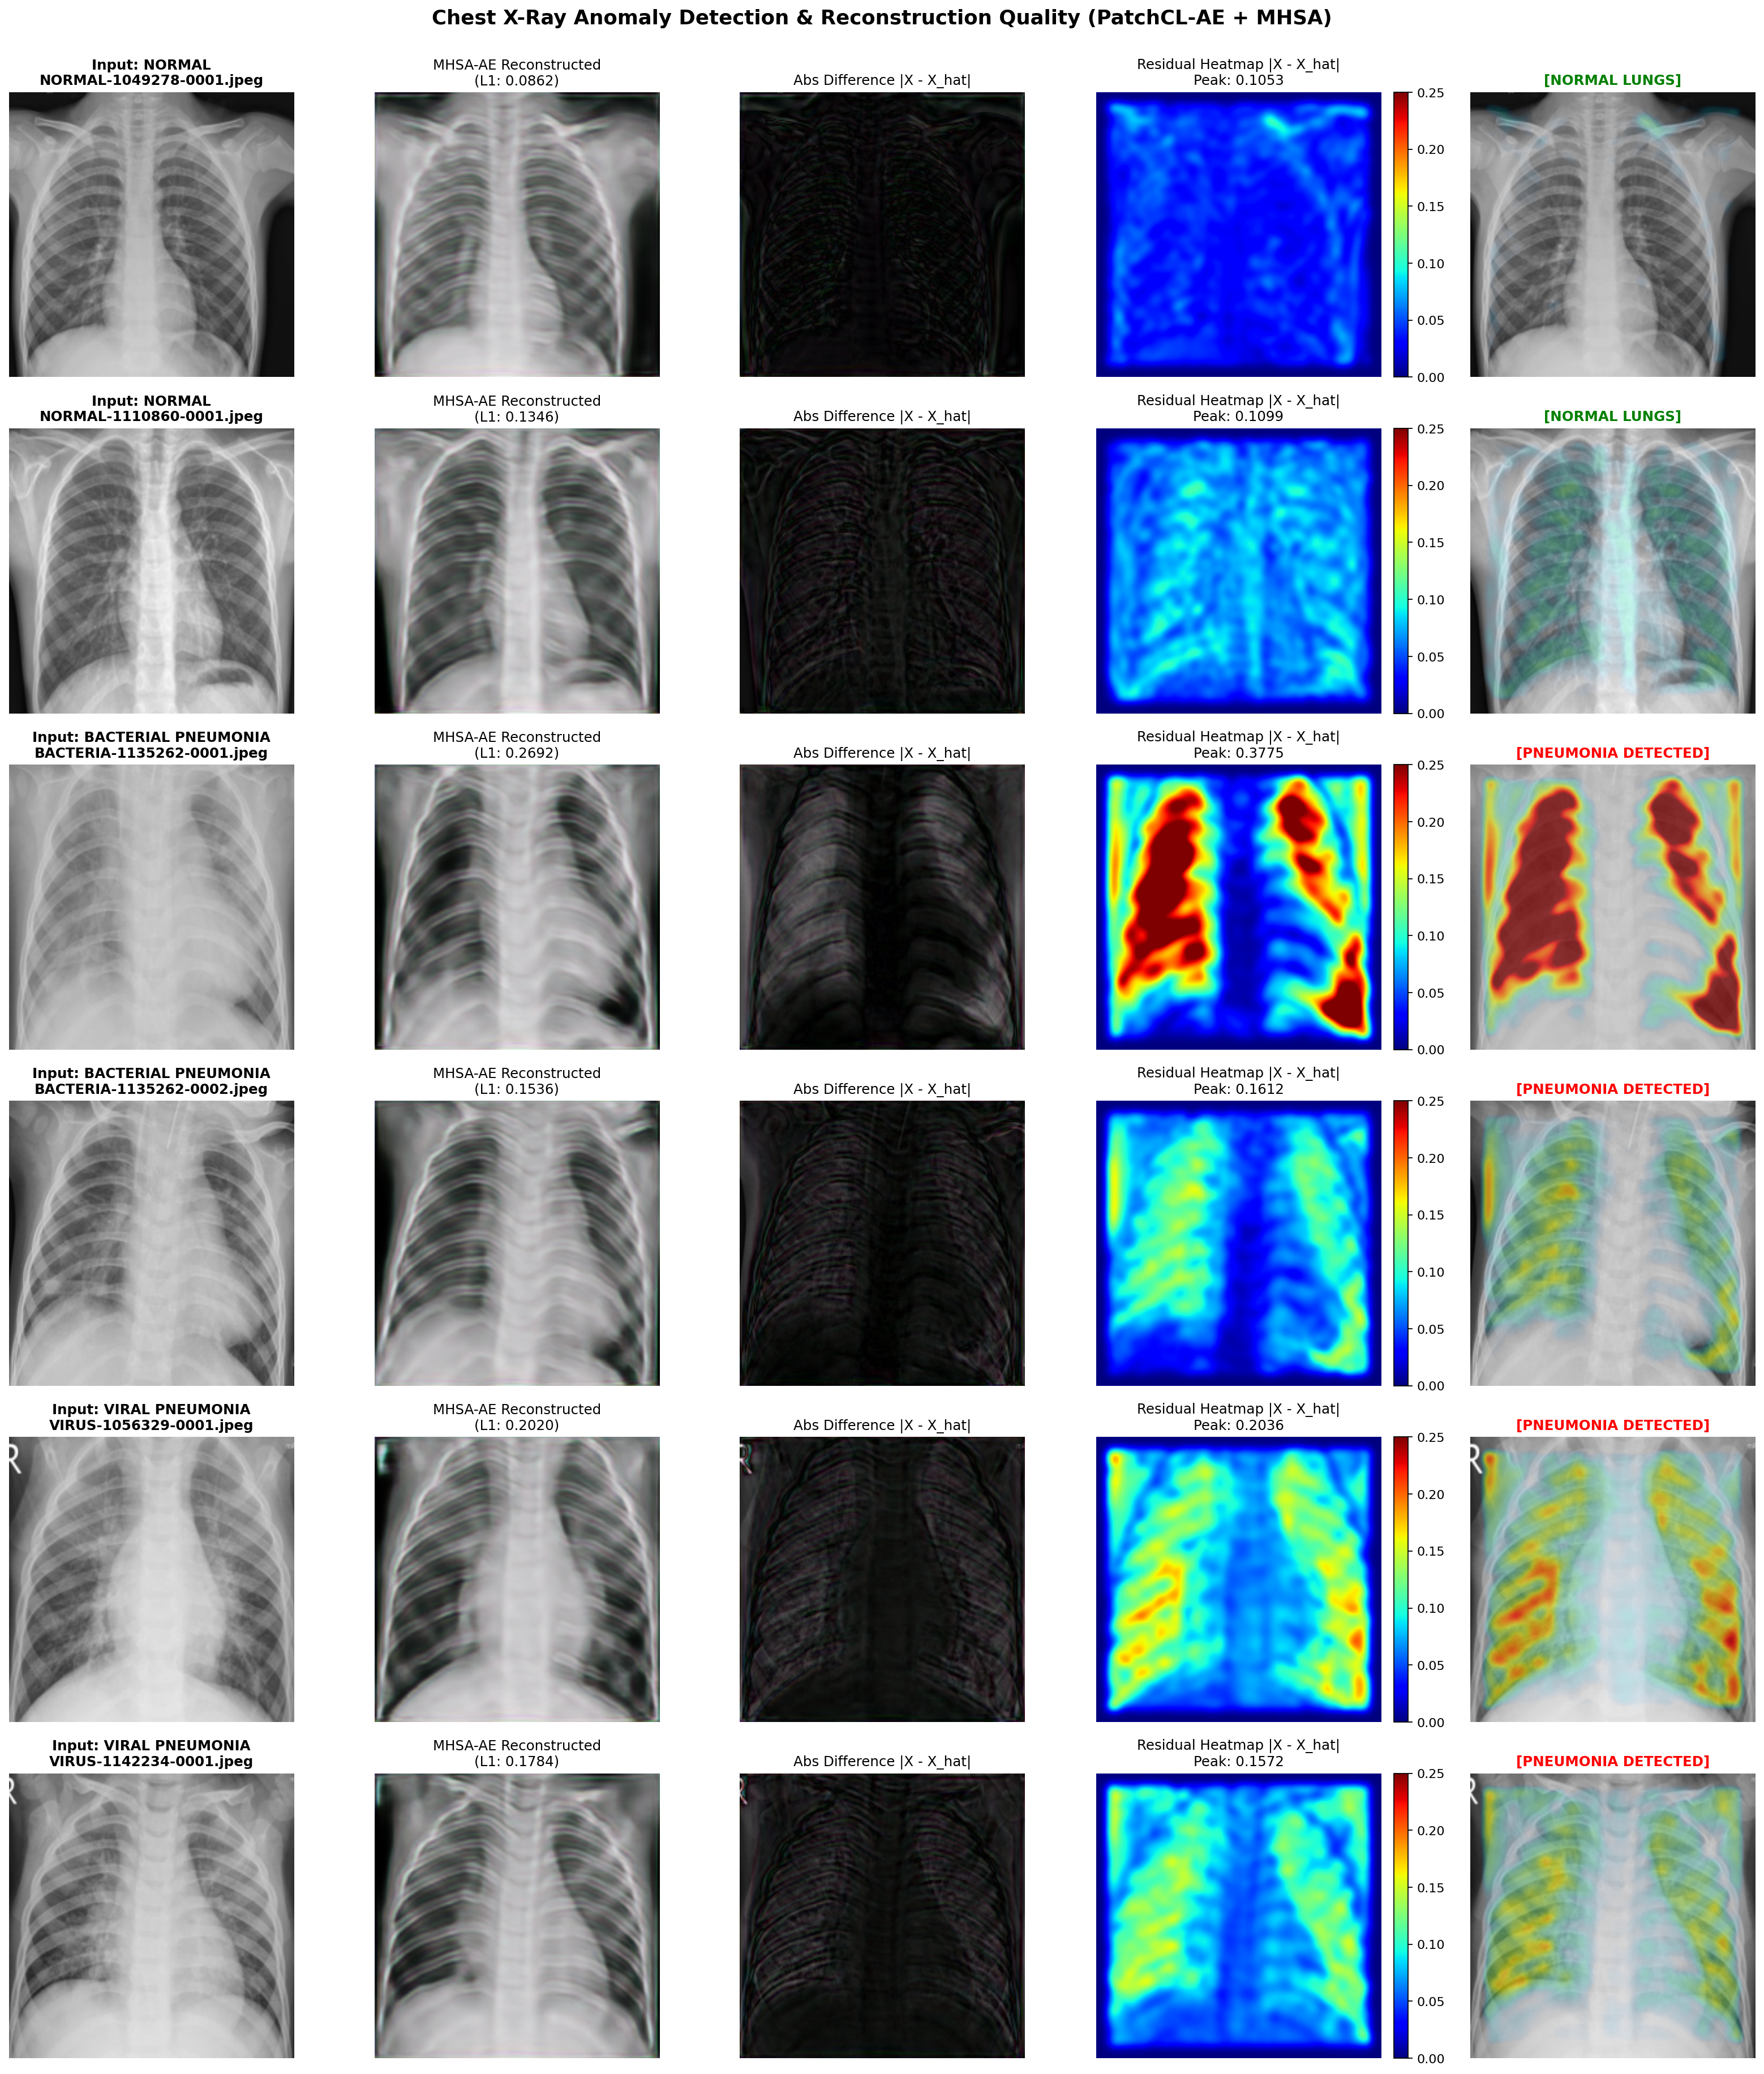
\includegraphics[width=\textwidth]{fig_chest_heatmap.png}
\caption{Qualitative anomaly detection performance on representative pediatric chest radiographs. Columns from left to right show the input radiograph, the reconstructed output from the proposed decoupled architecture, the absolute pixel difference, the synthesized multi-layer feature heatmap, and the corresponding diagnostic overlay.}
\label{fig:chest_results}
\end{figure*}

Fig.~\ref{fig:oct_results} presents qualitative evaluations across the four retinal conditions. The model effectively removes subretinal fluid accumulations in CNV and intraretinal cystoid cavities in DME, producing localized heatmap activations that align with pathological basement membrane disruptions.

\begin{figure*}[t]
\centering
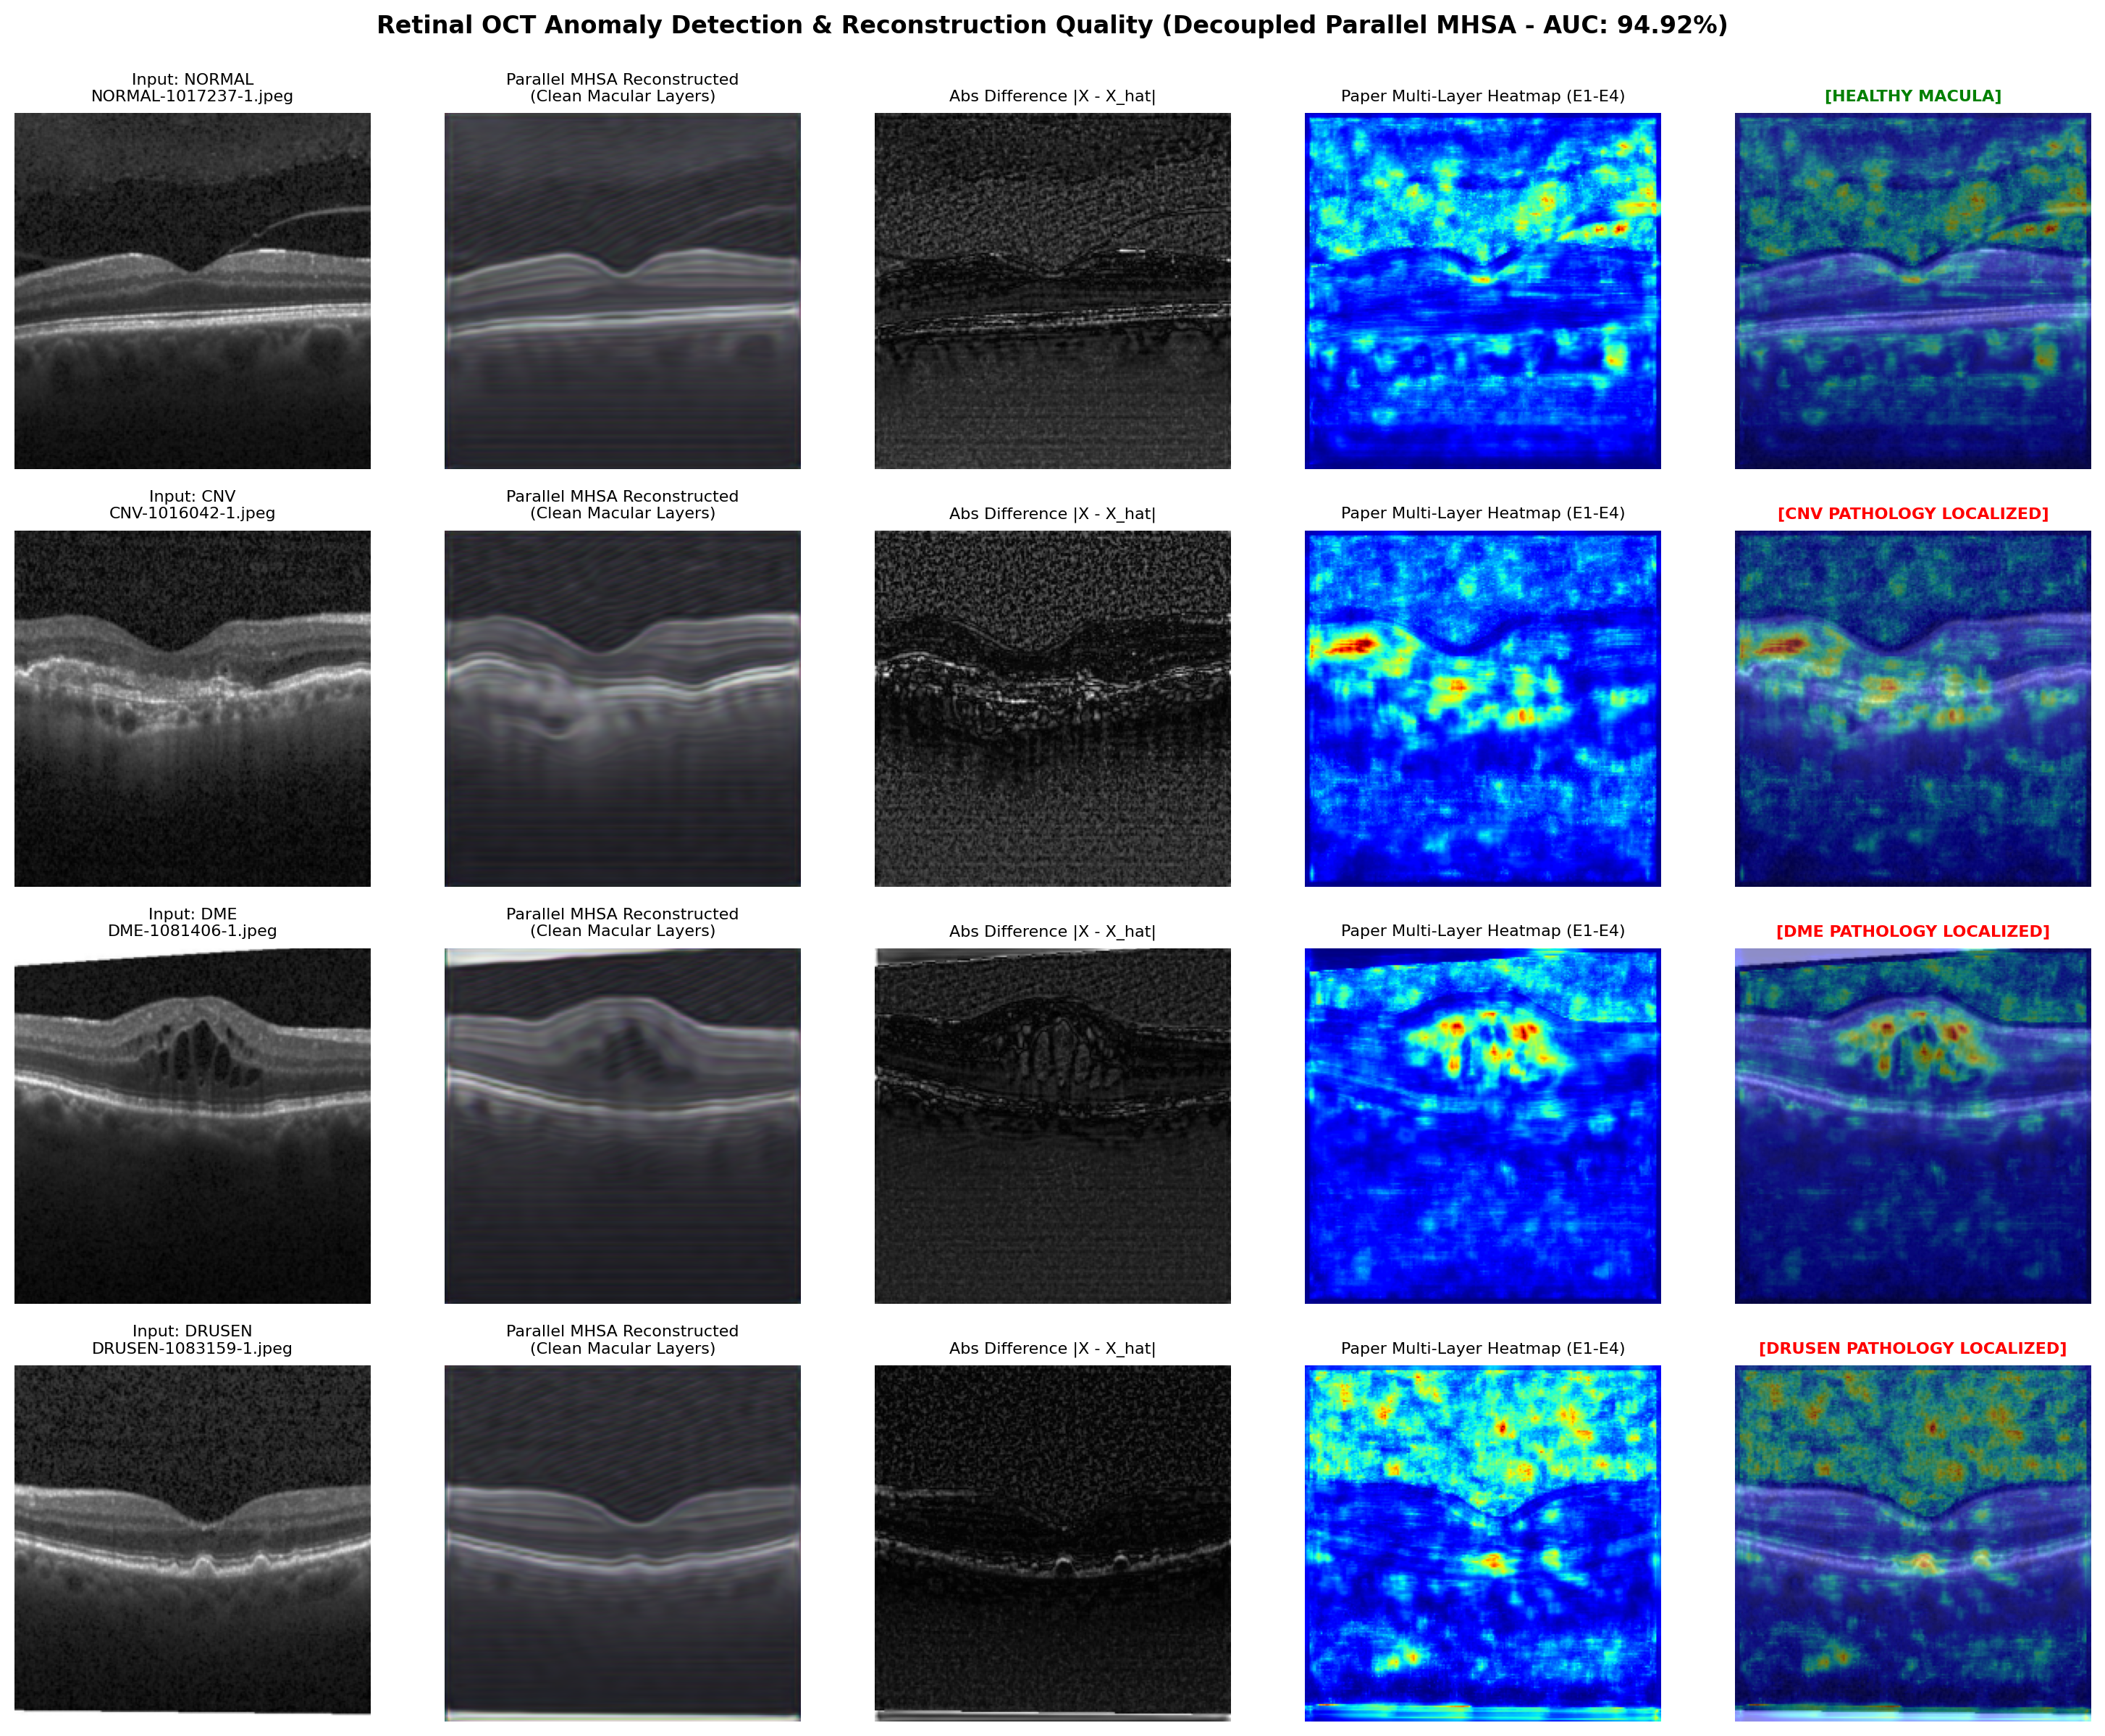
\includegraphics[width=\textwidth]{fig_oct_heatmap.png}
\caption{Qualitative visualization on the Retinal OCT2017 dataset across normal, choroidal neovascularization (CNV), diabetic macular edema (DME), and drusen examinations.}
\label{fig:oct_results}
\end{figure*}

Fig.~\ref{fig:pixel_residual} compares raw pixel-space residual maps with multi-scale feature distance maps. Direct pixel subtraction exhibits sensitivity to high-frequency skeletal contours along the clavicles and rib cage, whereas feature-space maps suppress non-pathological variations and isolate parenchymal consolidations.

\begin{figure}[t]
\centering
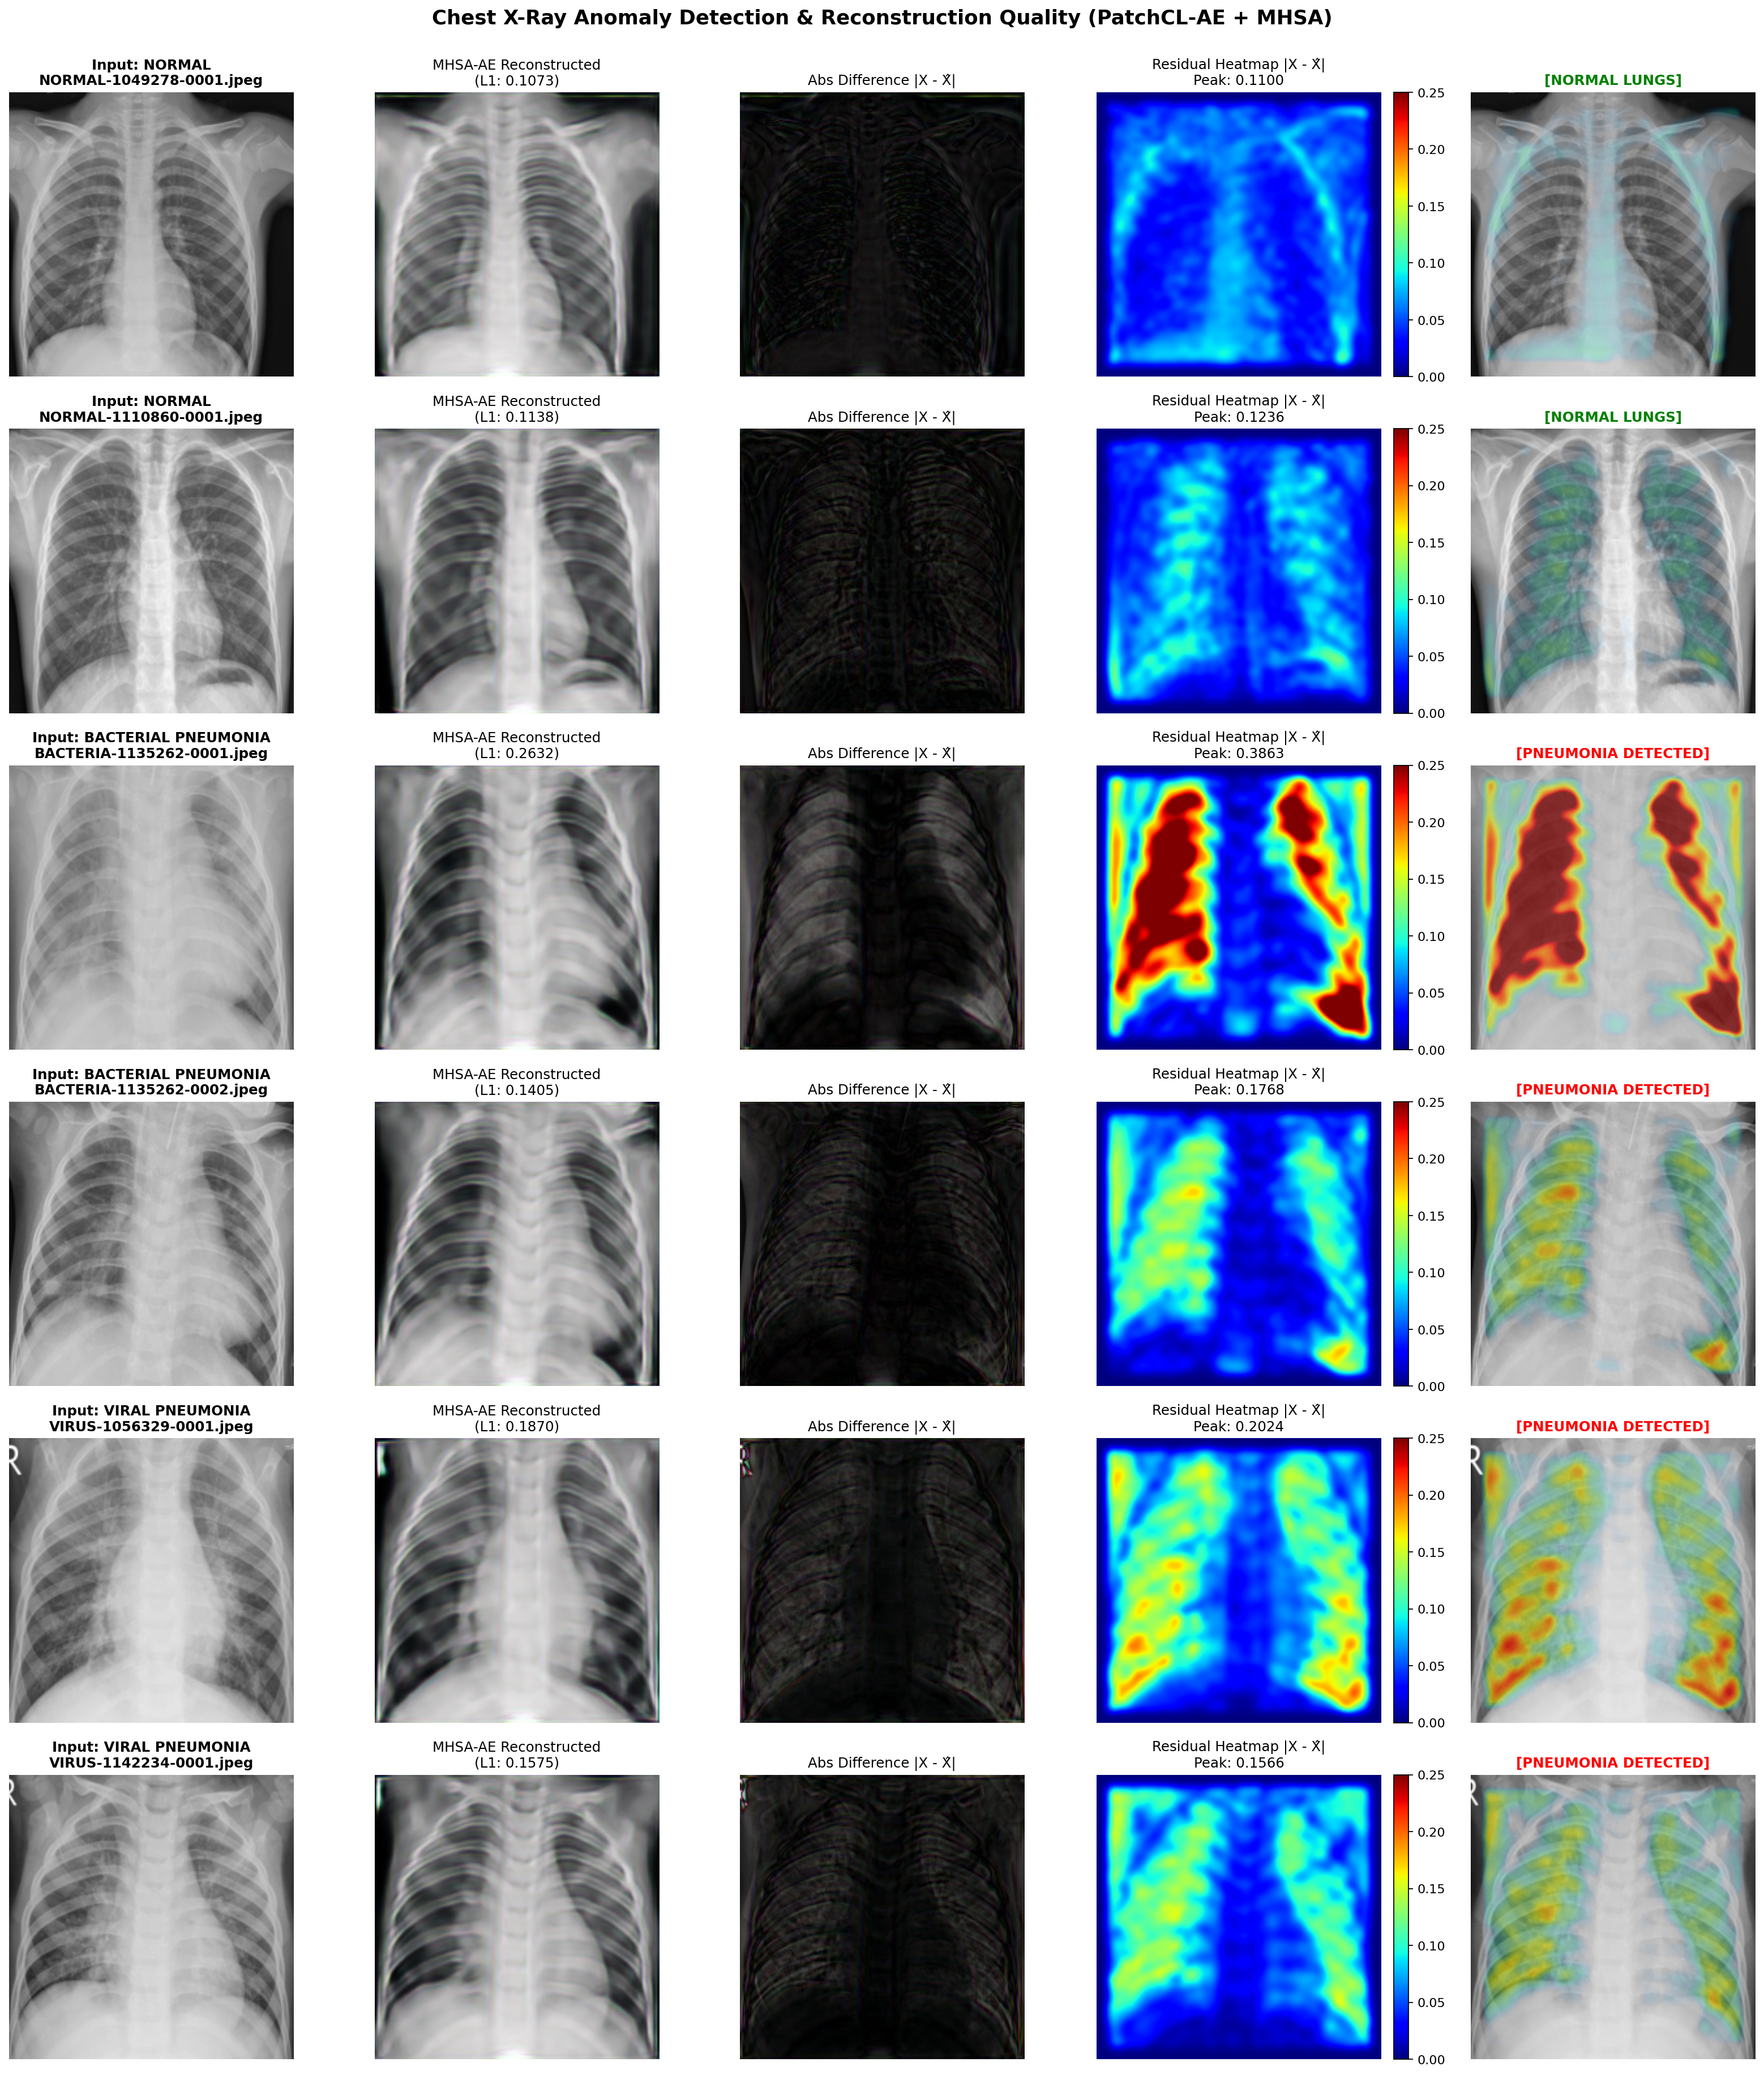
\includegraphics[width=\linewidth]{fig_pixel_residual.png}
\caption{Comparative visual analysis between direct pixel-level subtraction (left) and multi-layer feature cosine discrepancy (right) on chest examinations.}
\label{fig:pixel_residual}
\end{figure}

\section{Discussion and Future Work}
Clinical screening systems require balanced sensitivity and specificity to avoid overburdening healthcare personnel with unwarranted notifications. While the foundational PatchCL-AE architecture achieved notable progress in patch representation, its uniform negative sampling assumption imposed unintended penalties on anatomically symmetric healthy structures, lowering specificity on chest radiographs. By incorporating an attention-guided attenuation factor $w(i,j) = (1 - S_{ij})^\gamma$ within a decoupled parallel guidance stream, the proposed approach mitigates contralateral feature repulsion, elevating specificity to 81.62\% without compromising sensitivity on acute bacterial pneumonia.

On retinal optical coherence tomography, the decoupled framework demonstrates robust detection capability on exudative disorders, achieving 99.17\% sensitivity on choroidal neovascularization and 90.08\% on diabetic macular edema, alongside 94.63\% specificity on normal scans. In contrast, sensitivity on drusen examinations remains moderate at 50.00\%. Because drusen represent localized, non-exudative sub-retinal pigment epithelium deposits without fluid leakage, their subtle structural manifestations can blend into normal anatomical contours under downsampled feature representations.

In terms of future research directions, several avenues warrant exploration. Developing multi-scale wavelet attention mechanisms or dedicated high-resolution focal pathways could improve sensitivity toward subtle drusen deposits without disrupting normal basement membrane contours. Furthermore, extending the decoupled dual-stream formulation to three-dimensional volumetric modalities, such as computed tomography (CT) and magnetic resonance imaging (MRI), offers a promising direction for broader clinical translation.

\section{Conclusion}
This paper presented the decoupled dual-stream PatchCL-AE architecture for unsupervised medical image anomaly detection. By isolating a strictly constrained convolutional bottleneck from a parallel self-attention guidance branch, the framework resolves the bilateral false negative semantic collision inherent in symmetric medical imaging while preventing pathological reconstruction leakage. Experimental evaluations on pediatric chest radiographs and retinal optical coherence tomography scans demonstrate notable improvements in clinical specificity, robust lesion suppression, and clear diagnostic visualization, offering an effective foundation for computer-assisted medical screening.

\section*{Acknowledgment}
The authors would like to express their sincere appreciation to the Vietnam Aerospace University for supporting this research during the 2026--2027 academic year.

\bibliographystyle{IEEEtran}
\bibliography{references}

\begin{IEEEbiographynophoto}{Cao-Phuc Ha}
is currently pursuing the B.S. degree in artificial intelligence at FPT University, Vietnam. His research interests include computer vision, artificial intelligence, and robotics, with applications to autonomous vehicles, drones, and unmanned aerial systems. He aims to continue his academic journey toward a Ph.D. degree, focusing on the development of intelligent robotic systems and AI-driven perception technologies.
\end{IEEEbiographynophoto}

\begin{IEEEbiographynophoto}{Phu-Nguyen Le}
received a B.S. degree in electrical engineering from Da Nang University of Technology, Vietnam, in 2012, and the Ph.D. degree from the University of Ulsan, South Korea, in 2021. He is currently a lecturer with the Faculty of Electrical and Electronics Engineering, Vietnam Aerospace University, 104 Nguyen Van Troi Street, Phu Nhuan Ward, Ho Chi Minh City 700000, Vietnam. His research interests include sensor-based robotic applications, robot calibration, and AI-based robotic control.
\end{IEEEbiographynophoto}

\end{document}
